%----------------------------------------------------------------------
\section[Space Systems II]{Space Systems II}
%----------------------------------------------------------------------
 
%----------------------------------------------------------------------
\paragraph{Solar array and batteries sizing}
%----------------------------------------------------------------------

The most common electric power subsystem in a spacecraft is a combination of
solar arrays that serve as a primary power source to produce power, plus a set
of batteries as a secondary power source to store and manage power when  the
primary source is not available.

Solar arrays only convert a fraction of
the incoming solar power into electric power: inefficiencies depend on the
solar cell technology, the solar array geometry and temperature, the
orientation of the solar arrays with respect to the Sun, and the age of the
system (as solar cells degrade with time). All in all, we can write the
produced electric  power by the solar arrays (SA) as:
%
\begin{equation}
P_{SA} = \eta_{SA} A_{SA} S_{Sun}
\end{equation}
%
where:
%
\begin{itemize}
\item $\eta_{SA}$ is the overall solar array efficiency.
\item $A_{SA}$ is the area of the solar array.
\item $S_{Sun}$ is the solar irradiance at the spacecraft location, i.e. the 
power per unit area of the solar radiation. The SI units are W/m$^2$. 
For spacecraft orbiting the Earth, $S_{Sun}\simeq 1366$ W/m$^2$. If the 
spacecraft travels closer to the Sun (e.g. to Venus or Mercury), this number 
increases; if it travel away from the Sun (e.g. to Mars or Jupiter), this 
number decreases.
\end{itemize}
%

The solar arrays must produce electricity to power the spacecraft systems
during the sunlight period, and also to charge the batteries to sustain
power consumption during the eclipse. 
An Earth satellite spends some time in the sunlight and some time in eclipse
in each orbit. We can estimate the eclipse time in the case of a circular
orbit assuming that the shadow of the Earth is cylindrical away from the Sun,
and that the satellite track crosses fully this shade cylinder.
The angle $\theta$ in the figure is $\theta = \arcsin{R_E/(R_E+H)}$, where
$R_E$ is the radius of the Earth and $H$ the orbital altitude of the
spacecraft. The fraction of the orbit that the spacecraft is in eclipse
is then equal to $2\theta/(2\pi)$. For LEO satellites, this can be about
$1/3$ of the orbit.

%----------------------------------------------------------------------
\begin{center}
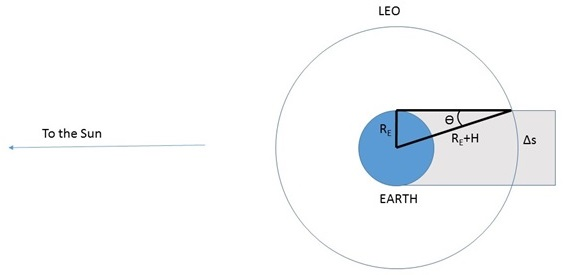
\includegraphics[width=0.6\textwidth]{figs/eclipse.jpg}
\end{center}
%----------------------------------------------------------------------

If a satellite requires an electric power $P$ continuously to operate,
then the solar arrays must provide a power
%
\begin{equation}
P_{SA} = P \frac{T_{orb}}{T_{light}}
\end{equation}
%
where $T_{orb} = 2\pi \sqrt{GM_E/(R_E +H)}$ is the orbital period, i.e., the
time it takes the satellite to complete one orbit, and $T_{light}$ is the
time spent in sunlight in one orbit.

In turn, the batteries must be sized so store and deliver every orbit the 
following energy:
%
\begin{equation}
E = P T_{eclipse}
\end{equation}
%
where $T_{eclipse}$ is the time spent in eclipse each orbit. Batteries must 
not undergo full charge/discharge cycles often, as this will severely limit
their durability. To extend the useful life of the batteries for the duration
of the spacecraft mission, we must limit the \emph{depth of discharge} (DOD) 
of the batteries to a given fraction that depends on the battery technology
and the number of charge/discharge cycles expected in the mission (i.e., the
total number of eclipses expected during the mission).
Once the design DOD is known, the actual energy of the batteries can be sized
as
%
\begin{equation}
E_{batt} = \frac{E}{DOD}.
\end{equation}

%----------------------------------------------------------------------
\paragraph{Thermal control in space}
%----------------------------------------------------------------------

In space, the only heat transfer mechanism that exists is radiation. Also,
within the spacecraft, conduction between the different, physically connected
parts, can transmit heat.

The balance between all the heat that is generated in one component $A$ by
dissipation of electric power, plus any heat coming from the surrounding space
environment and neighboring components into $A$, minus the heat that is
conducted or radiated away from $A$, is related to the rate at which the temperature of component $A$ changes in time:
%
\begin{equation}
C_A \frac{\dd T_A}{\dd t} = Q_{in,internal} + 
Q_{in,environment} - Q_{out}.
\end{equation}
%
In this thermal energy balance equation, $C_A$ is the thermal capacity of
the component $A$, i.e. how much heat must be provided to this component to 
make its temperature increase by a given amount. The SI units of $C_A$ are 
W/K.

Each component in the spacecraft has one such equation. The combination of all
these coupled equations can be solved simultaneously in a computer, to find the
evolution of the temperature of each component under different operating
conditions and environmental heat loads (eclipse, sunlight, etc).

If we consider an isolated component with no neighboring elements to conduct
or radiate heat to and from, the term $Q_{in,environment}$ represents the
incoming  radiation heat from space, and the term $Q_{out}$ represents the
outgoing radiation heat emitted from the object into space. Then, the external
heat sources from the environment are the solar radiation, the planetary
albedo (i.e. the reflection of solar radiation off the planet surface), and
the planetary IR radiation (i.e. the heat emitted by the planet itself since
it has a non-zero temperature). The background empty space can be considered 
to be at $4$ K, and can be ignored in most situations.
Of these loads, the Sun is the dominant one:
%
\begin{align}
Q_{in,environment} &= Q_{in,Sun} + Q_{in,albedo} + Q_{in,planet}
\\
Q_{in,Sun} &= \alpha_{Sun} A_\alpha S_{Sun}
\end{align}
%
where: 
%
\begin{itemize}
\item $\alpha_{Sun}$ is the solar absorptivity, i.e., what fraction of the 
incoming solar irradiance is absorbed by the component (the rest is reflected).
It is a non-dimensional number that ranges from 0 (no absorption) to 1 (
maximum absorption).
\item $A_\alpha$ is the effective area of absorption of the component that is 
exposed to sunlight.
\item $S_{Sun}$ is the solar irradiance at the spacecraft location as explained before, i.e. the 
power per unit area of the solar radiation. 
\end{itemize}
%

The heat emitted from tan isolated component is its radiation into space.
Since the component is typically at a few hundreds of degrees Kelvin, its
radiation is essentially in the infrared part of the spectrum, and the
emitted radiation heat can be expressed as:
%
\begin{equation}
Q_{out} = \varepsilon_{IR} A_\varepsilon \sigma T^4_A
\end{equation}
%
where:
%
\begin{itemize}
\item $\varepsilon_{IR}$ is the emissivity of the component in the infrared. 
It is a non-dimensional number that ranges from 0 (no emission) to 1 (maximum 
emission). The maximum emission is that of a so-called \emph{black body} at 
the same temperature as the object.
\item $A_\varepsilon$ is the effective area for radiation of the component.
\item $\sigma T^4_A$ is the power radiated as heat of a perfect black body at 
a temperature $T_A$. The Stefan-Boltzmann constant is 
$\sigma=5.67\cdot 10^{-8}$ W/(m$^2$K$^4$).
\end{itemize}
%

Different materials have different optical properties $\alpha_{Sun}$ and
$\varepsilon_{IR}$. By correctly selecting the materials of the surfaces of a
spacecraft, we can exert some control over its temperature when exposed to the
Sun and/or during eclipses (i.e. no Sun).
